
%\hypertarget{aula-14}{%
%\chapter{Aula: 14}\label{aula-14}}





\hypertarget{Roteadores.}{%
\chapter{Roteadores.}\label{Roteadores.}}

\hypertarget{analogia}{%
\section{Analogia}\label{analogia}}

Imagine uma via de veículos com pedágio. Suas entradas direcionam todos
os carros de diferentes origens para um mesmo pedágio. Durante o
pedágio, os carros aguardam pacientemente em uma fila a execução de uma
série de operações, como o pagamento da taxa de uso da via. Após essas
operações, os carros atravessam a via de transporte encaminhando-se até
as suas respectivas saídas.

O \emph{data plane} de um roteador funciona de forma análoga a essa via
imaginada. Os \emph{datagrams}, análogos aos carros, após entrarem no
roteador (pelos \emph{inputs}), são enfileirados e ficam no aguardo de
serem processados. Após uma série de operações, os mesmos são
direcionados para as suas respectivas saídas (\emph{outputs}).

Assim, o roteador é um caso específico da abstração mais genérica
\emph{match plus action} (corresponder e agir), o qual é performado
também por outros dispositivos, como os \emph{switches}, e não apenas
pelos roteadores.

A Figura \ref{Arquitetura de um roteador} apresenta a arquitetura de um roteador, separada em
\emph{control plane} e \emph{data plane}, que implementam o
\emph{routing} e o \emph{fowarding, respectivamente}.

\begin{figure}[h!]
\centering
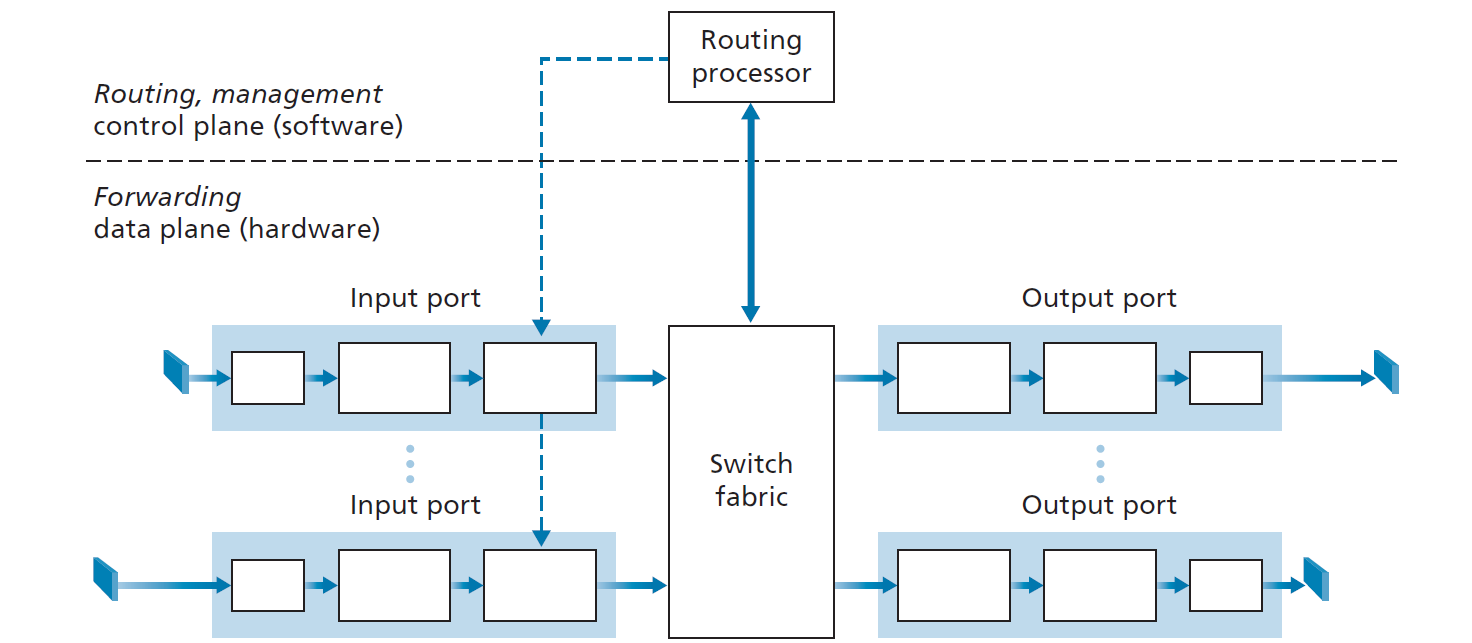
\includegraphics[keepaspectratio, width=14cm, height=11cm]{imagens/14/14 - Roteador.png}
\caption{Arquitetura de um roteador \\
Imagem retirada de: Computer Networking a top-down approach. 8th
ed.~Pearson, página 311. \\}
\label{Arquitetura de um roteador}
\end{figure}



\hypertarget{Descrição}{%
\section{Descrição}\label{Descrição}}

De forma mais descritiva, o roteador é composto por:

\begin{enumerate}
\def\labelenumi{\arabic{enumi}.}
\tightlist
\item
  \emph{input ports}: armazena os \emph{datagrams} recém chegados e
  performa funções da camada física e de enlace, como o \emph{lookup}, a
  determinação da porta de saída (para tal, é necessário consultar a
  \emph{fowarding table}).
\item
  \emph{Switching fabric}: conecta os \emph{input ports} com os
  \emph{Output ports}.
\item
  \emph{Output ports}: armazena os \emph{datagrams} recebidos pela
  \emph{Switching fabric} e transmite-os para fora do roteador
  (performando funções da camada física e de enlace essenciais).
\item
  \emph{Routing processor}: performa funções do \emph{control plane},
  como computar as rotas e manter a \emph{fowarding table} (em
  roteadores SDN, as operações mencionadas são feitas remotamente).
\end{enumerate}

É importante mencionar que os pontos 1, 2 e 3 são quase sempre
implementados em \emph{hardware}.

\hypertarget{tipos-de-forwarding}{%
\subsection{Tipos de forwarding}\label{tipos-de-forwarding}}

O \emph{output link} pode ser determinada de duas formas:

\begin{enumerate}
\def\labelenumi{\arabic{enumi}.}

\item
  \emph{Destination-based fowarding}: no qual a saída é baseada no
  destino.
\item
  \emph{Generalized forwarding}: em que o \emph{output link} é definido
  com base em N fatores, como a origem dos dados.
\end{enumerate}

Voltando para a analogia, o \emph{Destination-based fowarding} seria o
atendente do pedágio direcionar o carro a uma saída específica baseado
no destino que o motorista almeja. No caso do \emph{generalized
forwarding}, fatores como o tipo do veículo pode impactar na orientação
dada pelo atendente.

\hypertarget{questuxf5es-a-cerca-do-forwarding.}{%
\section{Questões a cerca do forwarding.}\label{questuxf5es-a-cerca-do-forwarding.}}

E se: 1. O atendente somente for capaz de atender 1 carro por minuto,
mas chegarem 2 carros por minuto ? 2. Todos os carros que entrarem forem
orientados para a mesma saída ? 3. Tiver mais carro entrando do que
saindo ? 4. For necessário tornar prioritário alguns veículos (como
ônibus) e bloquear a entrada de outros (como caminhões acima de um certo
peso) ?

Para as perguntas 1, 2 e 3, fica claro que gerará tráfego na entrada, na
saída e na via, respectivamente. Por fim, a resposta da pergunta 4 passa
pela criação de regras prévias a partir da definição das políticas de
filtro.

O mesmo pode ocorrer em um roteador, com a chegada de múltiplos
\emph{datagrams} em uma mesma \emph{input port} sendo maior que sua
capacidade de processá-los podendo gerar filas, atrasos e perda de dados
(com o mesmo ocorrendo na saída). A quantidade limitada de
\emph{datagrams} suportada pelo \emph{switch fabric} pode não suportar a
alta demanda de fluxo de dados, causando o bloqueio de novos entrantes
e, consequentemente, filas e atrasos.

Essas questões serão debatidas posteriormente em mais detalhes.

\hypertarget{input-port}{%
\section{Input Port}\label{input-port}}

A Figura \ref{Execuções na Input Port} mostra as execuções ocorridas na \emph{input port}.
Inicia-se com a ação de funções relativas a \emph{physical layer} (em
\emph{Line Termination}), seguida de funções da \emph{link layer} (em
\emph{Data link processing}), por fim o \emph{lookup, fowarding} e
\emph{queuing} (em \emph{lookup, fowarding, queuing}).





\begin{figure}[h!]
\centering
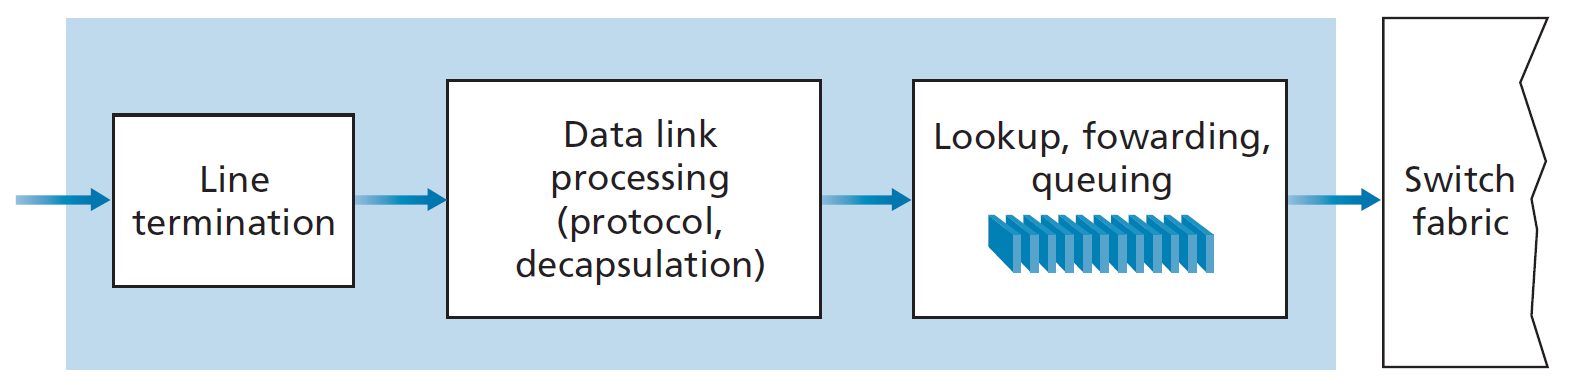
\includegraphics[keepaspectratio, width=12cm, height=9cm]{imagens/14/14 - input port.png}
\caption{Execuções na Input Port \\
Imagem retirada de: Computer Networking a top-down approach. 8th
ed.~Pearson, página 314. \\}
\label{Execuções na Input Port}
\end{figure}




A função central da porta de entrada é o \emph{lookup}, no qual o
roteador procura (\emph{look up}) na \emph{forwarding table} qual porta
o \emph{datagram} recém chegado deve ser direcionado. Apesar da
proeminente importância do \emph{lookup}, outras ações também devem ser
tomadas, como a checagem do \emph{version number}, \emph{checksum} e
\emph{Time to Live}

Como pode-se supor, em uma arquitetura de banco de dados centralizado,
os registros da \emph{forwarding table} estariam disponíveis em um único
local do roteador, com a operação de \emph{look up} devendo fazer uma
requisição de registro à esse banco de dados, algo que gera um possível
gargalo, afinal, caso o módulo do banco de dados não conseguir suprir a
demanda das requisições, deverão ocorrer filas e atrasos.

Para evitar esse gargalo, cada linha da tabela é copiada para cada um
dos \emph{input ports} presentes no roteador, de forma que o acesso à
tabela de transmissão (\emph{forwarding table}) seja feita localmente
(no \emph{input port}), sem a necessidade de requisições.

No \emph{look up}, o roteador identifica a saída (\emph{link interface})
utilizando a regra de maior correspondência (\emph{longest prefix
matching rule}) de prefixo do IP \emph{Address} de destino do
\emph{datagram}. Um exemplo dessas correspondências podem ser vistas na
Tabela 01. (O prefixo é formado por x primeiros dígitos do IP
\emph{Address} de destino referencia o endereço da sub-rede.)


\begin{table}[h!]
\centering
\begin{tabular}{||c c||} 
 \hline
    Prefix & Link Interface \\ [0.5ex] 
 \hline\hline
    11001000 00010111 00010 & 0 \\
 \hline
    11001000 00010111 00011000 & 1 \\
 \hline
    11001000 00010111 00011 & 2 \\
 \hline
    Prefix & Link Interface \\
 \hline

\end{tabular}
\caption{Exemplo de forwarding table \\}
\label{Exemplo de forwarding table}
\end{table}




Por exemplo, o endereço de IP:

\begin{verbatim}
11001000 00010111 00011000 10101010
\end{verbatim}

Tem o prefixo correspondendo ao \emph{link interface} 1 e 2, com o
\emph{link} 1 sendo a maior correspondência e, portanto, sendo os dados
direcionados ao mesmo.

\hypertarget{switching}{%
\section{Switching}\label{switching}}

O \emph{switching fabric} tem a função de conectar as \emph{input ports}
com as \emph{output ports}. Há diferentes formas de implementá-lo, mas
três delas, mostradas na Figura \ref{Tipos de Switching}, destacam-se:


\begin{figure}[h!]
\centering
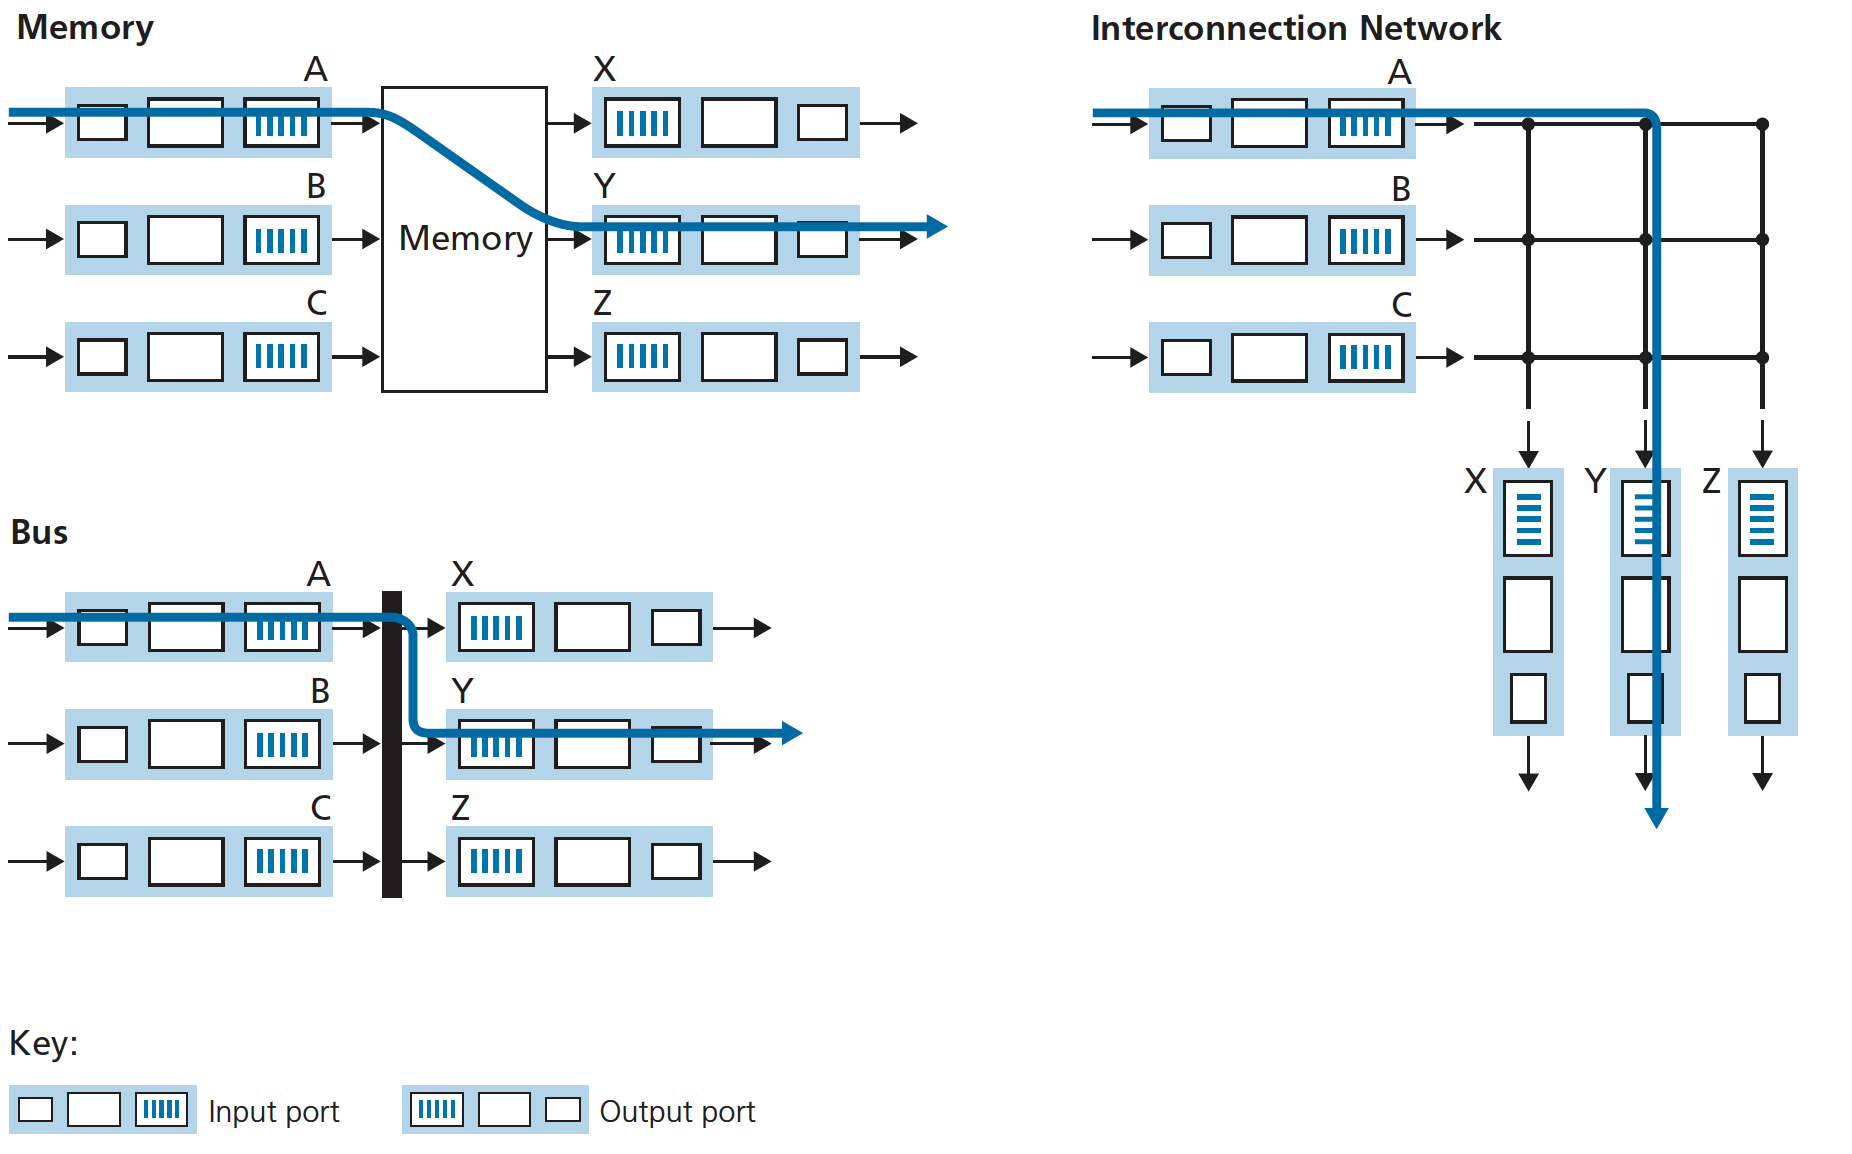
\includegraphics[keepaspectratio, width=16cm, height=13cm]{imagens/14/14 - switching.png}
\caption{Tipos de Switching \\
Imagem retirada de: Computer Networking a top-down approach. 8th
ed.~Pearson, página 317. \\}
\label{Tipos de Switching}
\end{figure}



\begin{enumerate}
\def\labelenumi{\arabic{enumi}.}

\item
  \emph{Switching via memory}: o \emph{input port} sinaliza, a partir de
  uma interrupção, para o processador do roteador a chegada de novos
  \emph{datagrams}. Após a interrupções, os dados recém chegados são
  copiados para a memória, processados (determinando-se a interface
  apropriada), e por fim copiados para o \emph{buffer} de saída. Isso é
  usualmente feito com processos com memória compartilhada.Como
  desvantagem pode-se citar, primeiro, a impossibilidade de transmissão
  de mais de um \emph{datagram} ao mesmo tempo, pois somente uma
  operação de leitura e escrita na memória pode ser feita por vez.
  Segundo, com a largura de banda sendo B \emph{datagrams} por segundo
  para memória (B \emph{datagrams} podem ser escritos ou lidos em 1
  segundo), significa dizer que a taxa de transferência está limitada em
  B/2 (pois será necessário fazer 1 operação de escrita e uma de
  leitura).
\item
  \emph{Switching via bus}: a \emph{input port} envia os
  \emph{datagrams} diretamente para a sua respectiva \emph{output port}
  através de um barramento compartilhado, sem a intervenção do
  processador do roteador. Isso é usualmente feito agregando-se um
  \emph{header} com um rótulo informando sua respectiva interface. Ao
  ser transmitido, todas as interfaces recebem esses dados, porém
  somente aquela indicada pelo rótulo irá manter o mesmo, retirando o
  seu rótulo, processando-o, e transmitindo-o para fora do roteador. O
  primeiro fato inconveniente dessa arquitetura é que somente 1 pacote de
  dados podem pecorrer o barramento. Isso significa que se chegarem
  múltiplos \emph{datagrams} em diferentes \emph{input ports}, todos
  menos 1 devem esperar o barramento tornar-se disponível. O segundo
  problema é que a velocidade do roteador estará limitada pela
  velocidade do barramento barramento. Esse tipo de arquitetura é
  indicado para LAN.
\item
  \emph{Switching via an interconnection network}: também chamado de
  cruzamento de barras, esse tipo de switch, como mostrado na Figura 02,
  pode alternar cada cruzamento de barra (ou nó) entre aberto e fechado
  de forma independente. Dessa maneira, multiplos \emph{datagrams} podem
  atravessar em paralelo o \emph{switch fabric} ao mesmo (ou seja,
  \emph{non-blocking} para uma \emph{output port} específica). Por
  exemplo, para emitir um dado do \emph{input} A para o \emph{output} Y,
  basta fechar o cruzamento dos mesmos. Esse fechamento não impedirá que
  os dados do \emph{input} B alcance a saída X, porém o \emph{output} Y
  estará somente disponível para o \emph{input} A (estando bloqueado
  para os outros \emph{inputs}).
\end{enumerate}

\hypertarget{output-port}{%
\section{Output port}\label{output-port}}

A Figura \ref{fig:Output Port} mostra as 3 principais execuções do \emph{output port}.
Inicia-se com o enfileiramento (\emph{Queuing}) dos \emph{datagrams}
recebidos. Em seguida, são performados ações necessárias relativas as
camadas físicas e enlace (\emph{Data link processing}). Por fim, os
dados são enviados para fora do roteador (\emph{Line termination}).


\begin{figure}[h!]
\centering
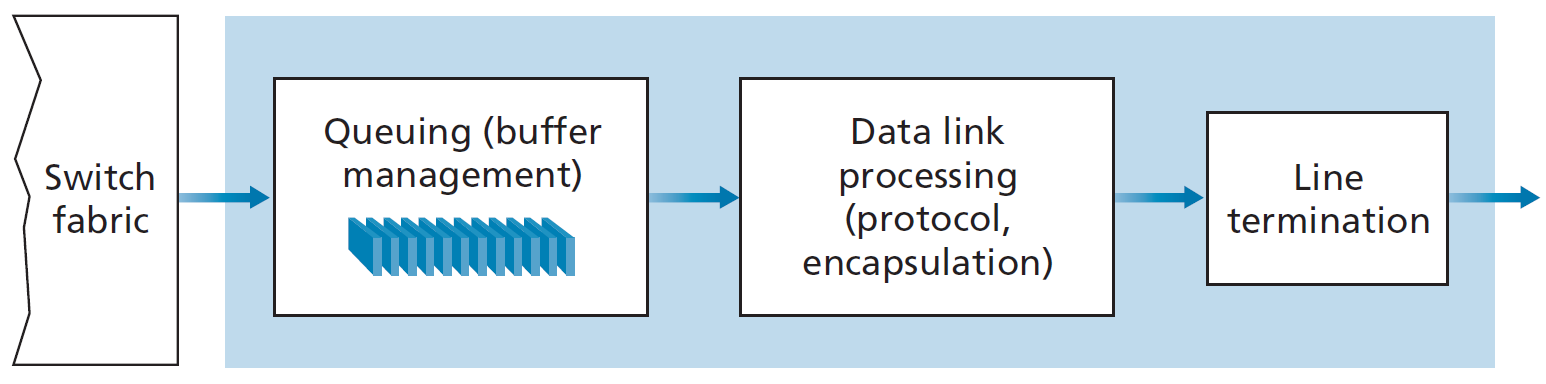
\includegraphics[keepaspectratio, width=12cm, height=9cm]{imagens/14/14 - output port.png}
\caption{Output Port \\
Imagem retirada de: Computer Networking a top-down approach. 8th
ed.~Pearson, página 319. \\}
\label{fig:Output Port}
\end{figure}


\hypertarget{filas}{%
\section{Filas}\label{filas}}

As filas podem se formar na entrada e na saída do roteador.

As filas na entrada podem ser formadas pela diferença de velocidade
entre o \emph{input} e o \emph{switching fabric} (como citado
anteriormente, de forma análoga, na questão 1 do ``E se'' no tópico''
Questões a a cerca do forwarding''). Se um \emph{input} for capaz de
lidar com uma taxa de \emph{datagrams} mais alta do que o
\emph{switching fabric}, os mesmos ficarão acumulados na entrada até
serem executados pelo \emph{switching fabric}.

Um outro evento que têm como consequência a geração de filas é o chamado
\emph{head-of-the-line blocking} (HOL \emph{blocking}). A Figura \ref{fig:Hol Blocking}
mostra um exemplo de como o HOL \emph{blocking} pode ocorrer. Os
\emph{datagrams} azuis-escuros estão destinados às saídas superiores,
enquanto que os azuis-claros estão destinados às saídas centrais. Assim,
um azul-escuro oriundo do \emph{input} superior pode bloquear a passagem
do \emph{datagram} azul-escuro oriundo do \emph{input} inferior,
travando a fila e impedindo que o \emph{datagram} azul-claro seja
processado paralelamente, apesar do caminho até sua saída estar livre.


\begin{figure}[h!]
\centering
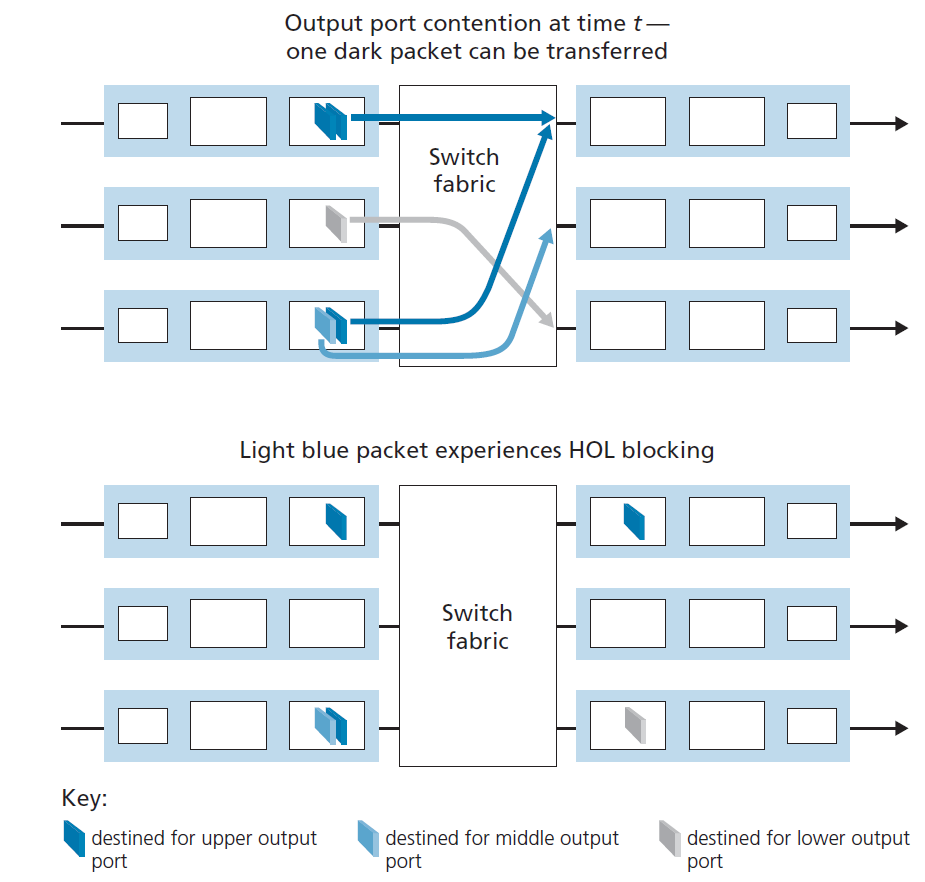
\includegraphics[keepaspectratio, width=14cm, height=11cm]{imagens/14/14 - hol blocking.png}
\caption{Hol Blocking \\
Imagem retirada de: Computer Networking a top-down approach. 8th
ed.~Pearson, página 321. \\}
\label{fig:Hol Blocking}
\end{figure}


Na saída, as filas podem se formar quando múltiplos \emph{datagrams} dos
\emph{inputs} são direcionados para o mesmo \emph{output}, como mostrado
na Figura \ref{fig:Fila na saída}. Esse evento pode preencher o \emph{buffer} de saída,
ocasionando a ``derrubada'' de novos \emph{datagrams}, política chamada
de \emph{drop-tail}, ou a remoção de um já enfileirado, para assim criar
espaço para os dados recém chegados. Em alguns casos, pode ser vantajoso
remover um pacote de dados antes que fila fique cheia, de forma a enviar
um sinal de congestionamento para o emissor. Os algoritmos responsáveis
por isso são chamados de \emph{Active Queue Management} (AQM), ou
gerenciador de filas ativo, com o \emph{Random Early Detection} (RED)
sendo um algoritmo dessa classe amplamente implementado.


\begin{figure}[h!]
\centering
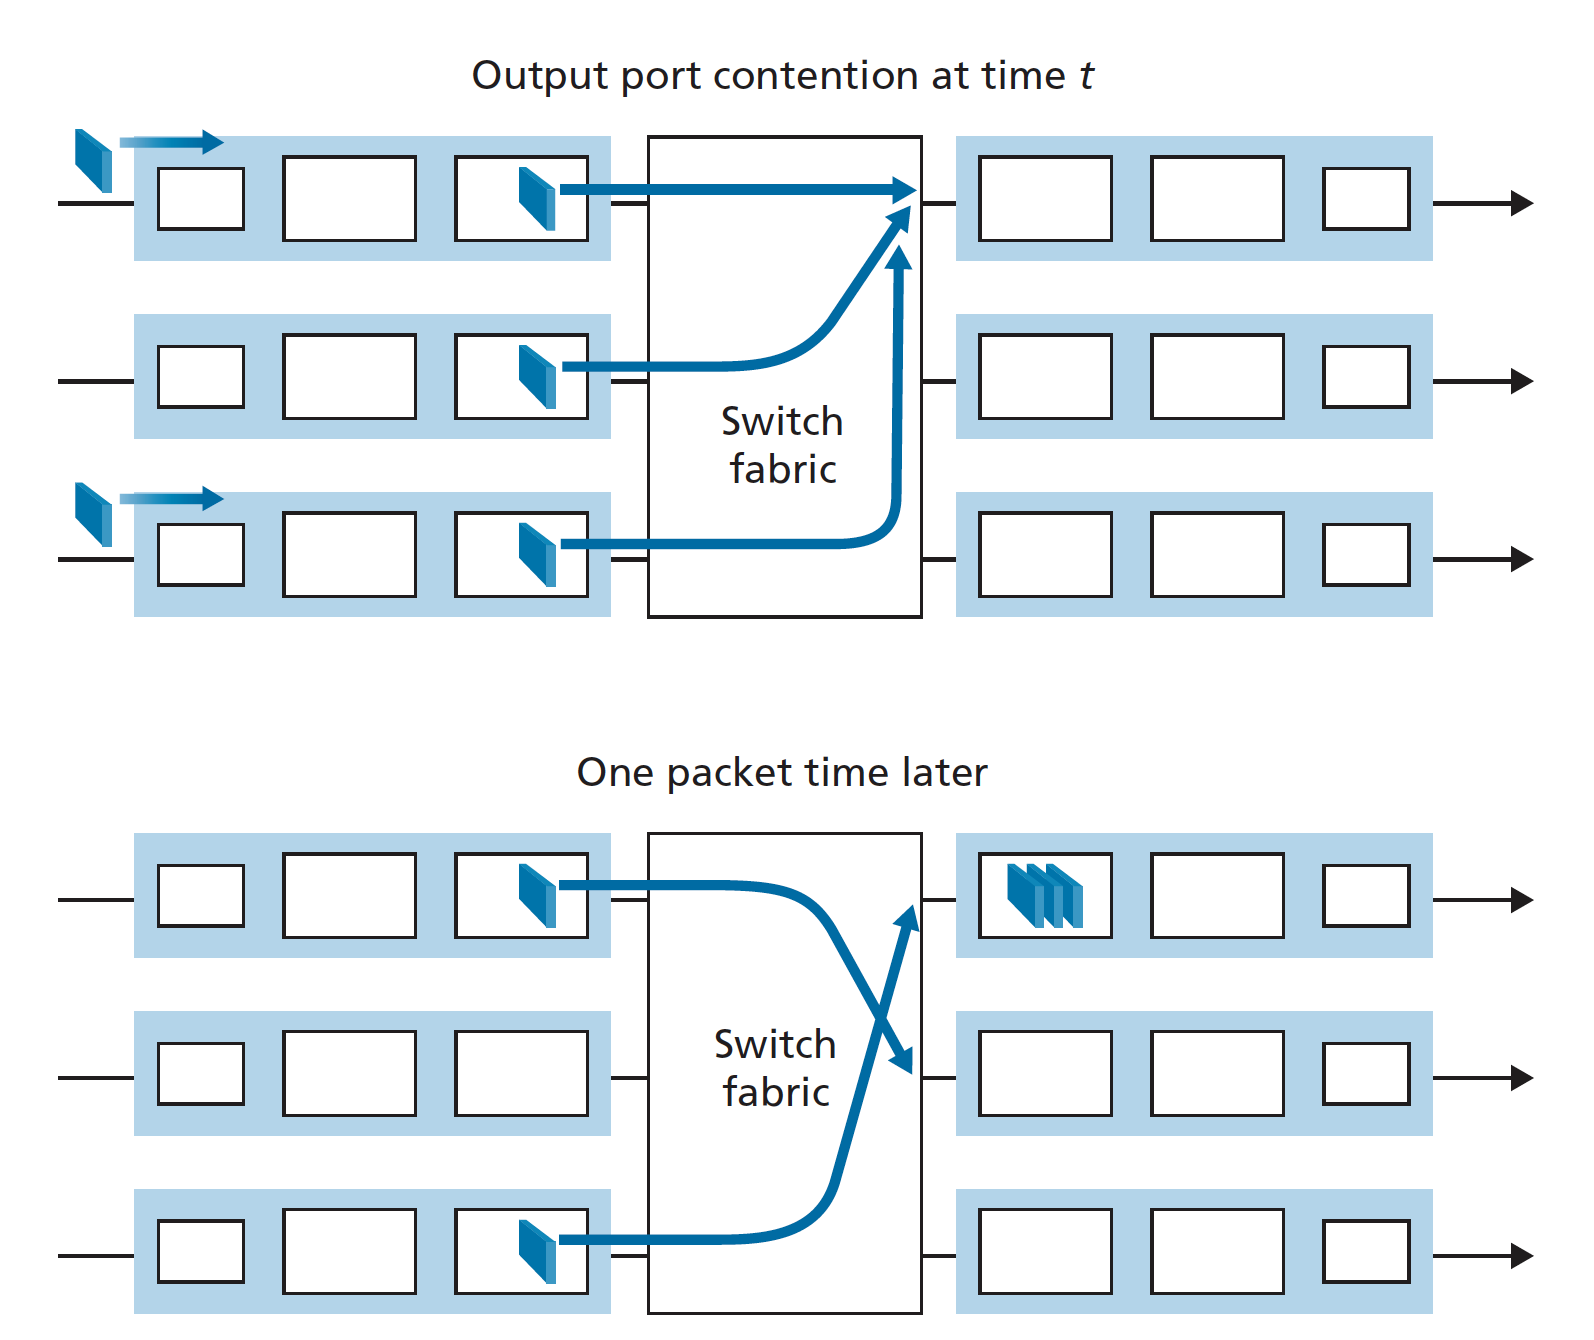
\includegraphics[keepaspectratio, width=12cm, height=9cm]{imagens/14/14 - output queue.png}
\caption{Fila na saída \\
Imagem retirada de: Computer Networking a top-down approach. 8th
ed.~Pearson, página 322. \\}
\label{fig:Fila na saída}
\end{figure}




O tamanho do espaço destinado para as filas sofrem de uma dicotomia.
Enquanto que \emph{buffers} pequenos podem não apresentar espaço
suficiente para lidar com picos de demanda, algo que aumenta o número de
dados perdidos, filas grandes podem representar um longo tempo de
espera, aumentando o atraso na entrega dos \emph{datagrams}.

Para equilibrar esses diferentes pontos, o tamanho do \emph{buffer}
(\texttt{B}) fora relacionado com o \emph{round-trip time} (RTT) médio
(período entre a emissão dos dados e a recepção do seu ACK) e a
capacidade do link (\texttt{C}).

\begin{verbatim}
B = RTT . C

B = 2.5G bits, para RTT = 250 ms, e C = 10 Gbps
\end{verbatim}

Atualmente, também relaciona-se o número de fluxos independentes de TCP
(\texttt{N}):

\begin{verbatim}
B = RTT . C / sqrt{N} 
\end{verbatim}

\hypertarget{prioridades-dos-dados}{%
\section{Prioridades dos dados}\label{prioridades-dos-dados}}

Na discussão dos \emph{buffers} fora deixado implícito a política
\emph{First-in-First-Out} (FIFO), ou primeiro a chegar, primeiro a sair
(modelo mostrado na Figura \ref{fig:Modelo FIFO}), mas outras regras também podem ser
utilizadas, como a classificação dos dados em diferentes filas a partir
de sua prioridade (modelo mostrado na Figura \ref{fig:Modelo classificação e priorização}).


\begin{figure}[h!]
\centering
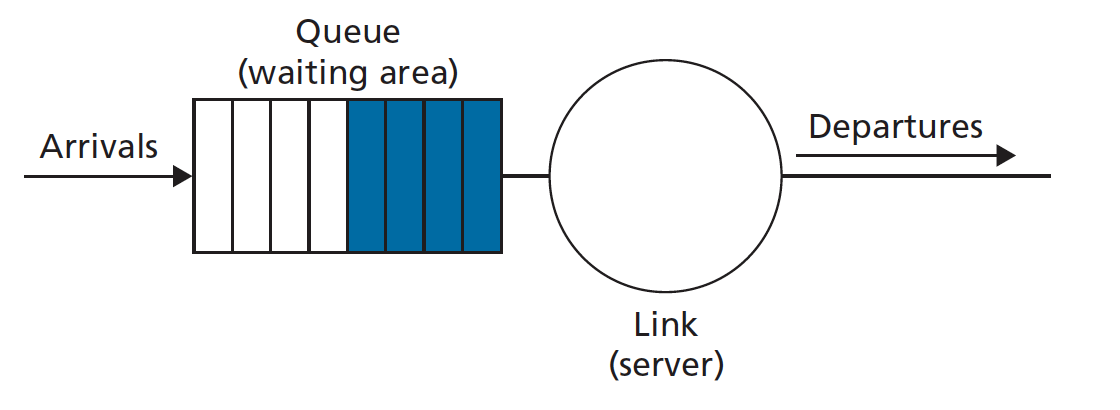
\includegraphics[keepaspectratio, width=12cm, height=9cm]{imagens/14/14 - FIFO.png}
\caption{Modelo FIFO \\
Imagem retirada de: Computer Networking a top-down approach. 8th
ed.~Pearson, página 325. \\}
\label{fig:Modelo FIFO}
\end{figure}




\begin{figure}[h!]
\centering
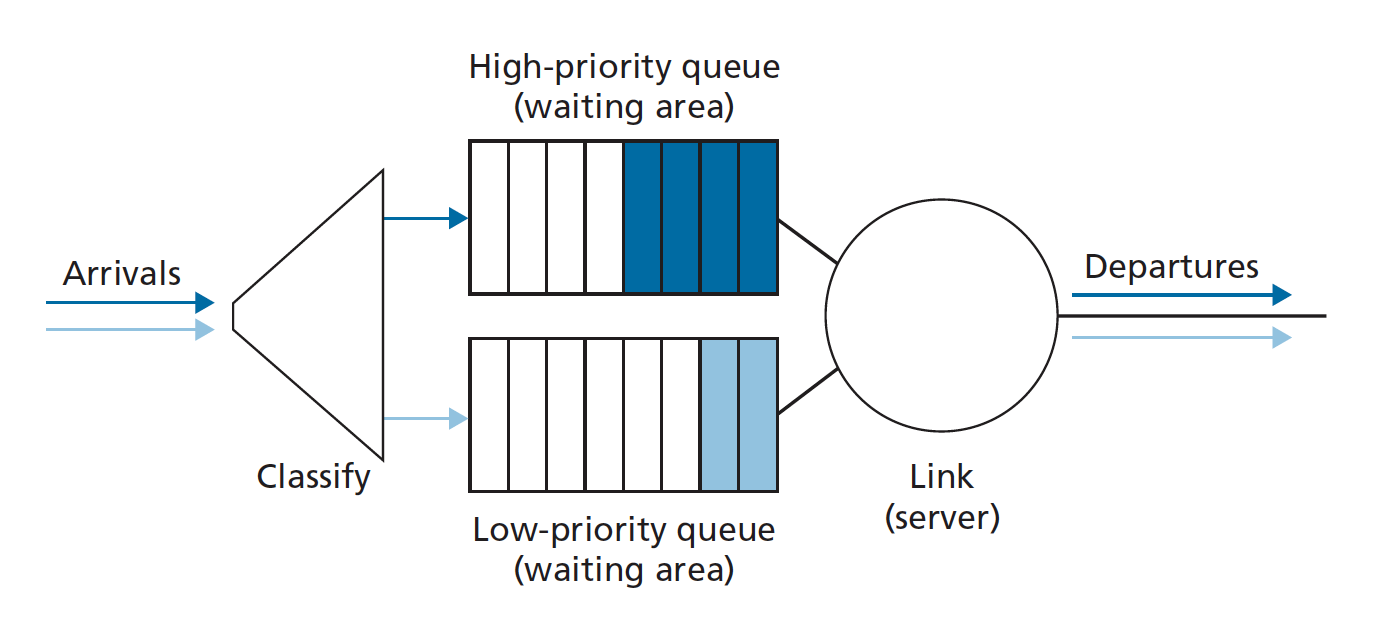
\includegraphics[keepaspectratio, width=12cm, height=9cm]{imagens/14/14 - priority queue.png}
\caption{Modelo classificação e priorização \\
Imagem retirada de: Computer Networking a top-down approach. 8th
ed.~Pearson, página 326. \\}
\label{fig:Modelo classificação e priorização}
\end{figure}

Uma forma generalizada de classificação e priorização dos dados que tem
sido bastante implementada é o chamada de \emph{Weighted Fair Queuing}
(WFQ), na qual as filas de maior peso são tratadas primeiro, seguindo
para as de menor peso, até reiniciar o ciclo, como mostrado na Figura
\ref{fig:Weighted Fair Queuing}.


\begin{figure}[h!]
\centering
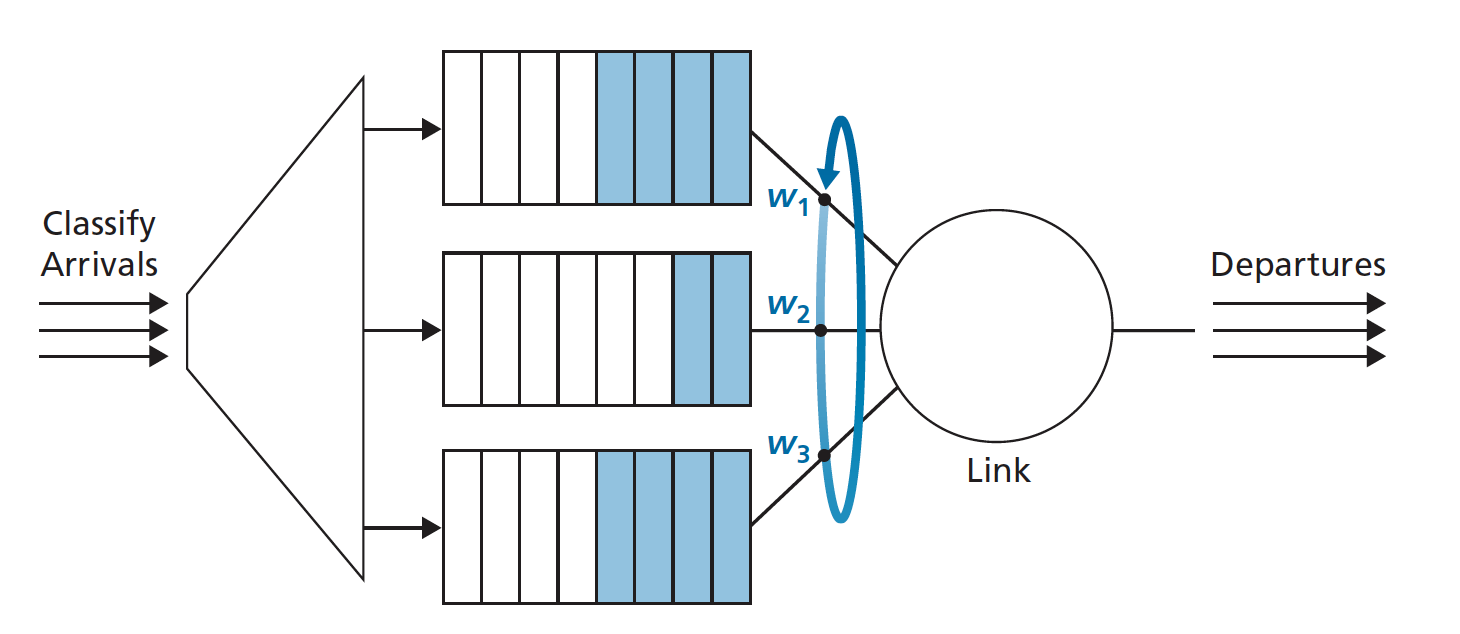
\includegraphics[keepaspectratio, width=12cm, height=9cm]{imagens/14/14 - WFQ.png}
\caption{Weighted Fair Queuing \\
Imagem retirada de: Computer Networking a top-down approach. 8th
ed.~Pearson, página 326. \\}
\label{fig:Weighted Fair Queuing}
\end{figure}



\hypertarget{neutralidade-das-redes}{%
\subsection{Neutralidade das redes}\label{neutralidade-das-redes}}

Como qualquer regra pode ser imposta para a classificação dos dados, os
ISP's podem não ser neutros no oferecimento de seus serviços, algo que
vem resultando leis que regulamentam o que os ISP's podem ou não fazer.

Em geral, a defesa da neutralidade das redes pode ser resumido em 3
pontos:

\begin{enumerate}
\def\labelenumi{\arabic{enumi}.}
\tightlist
\item
  Conteúdos não devem ser bloqueados (\emph{No Blocking}).
\item
  Tráfico de Internet não deve ser penalizado (\emph{No Throttling}).
\item
  Não deve haver priorização paga (\emph{Paid Prioritization}).
\end{enumerate}

\hypertarget{generalized-forwarding}{%
\chapter{Generalized Forwarding}\label{generalized-forwarding}}

O \emph{Generalized Forwarding} é a forma genérica do paradigma
\emph{match plus action}, no qual utiliza os \emph{headers} associados
aos protocolos de diferentes camadas para determinar o que deve ser
feito com os dados recebidos. Para a sua implementação, é utilizado o
padrão OpenFlow, o qual baseia-se no SDN (\emph{Software Defined
Network}), que aplica um controlador remoto para o cálculo das regras da
rede.

A base do \emph{Generalized Forwarding} está na \emph{Flow Table},
tabela no qual está contido as regras do \emph{match plus action}. Cada
regra têm:

\begin{enumerate}
\def\labelenumi{\arabic{enumi}.}
\tightlist
\item
  Um conjunto de \emph{headers} à serem verificados.
\item
  Um conjunto de contadores.
\item
  Um conjunto de ações à serem tomadas.
\end{enumerate}

Perceba que essa tabela é uma forma limitada de programação. Atualmente,
vem ganhando força uma alternativa mais rica de possibilidades de
implementação (com variáveis e funções), a linguagem \emph{Programming
Protocol-independent Packet Processors} (P4).

Dentro do padrão OpenFlow, os \emph{headers} podem ser oriundos das
camadas de enlace, rede e transporte, como mostrado na Figura \ref{fig:OpenFlow Headers}. É
importante perceber que nem todos os \emph{headers} podem ser escolhidos
para a ação de correspondência (\emph{match}) (assim fora implementado
como uma forma de equilibrar a funcionalidade e complexidade. É melhor
fazer algo simples e bem, do que muita coisa e ruim).


\begin{figure}[h!]
\centering
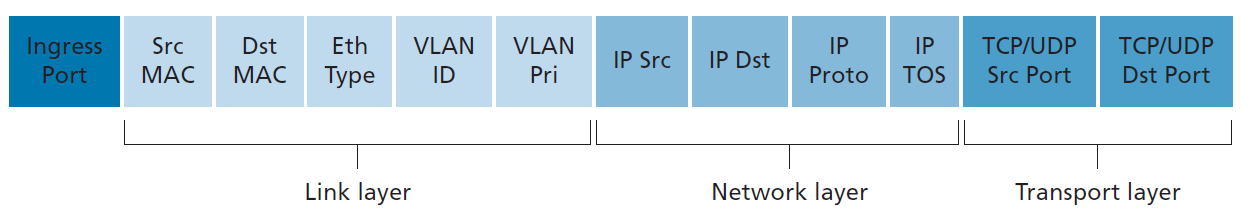
\includegraphics[keepaspectratio, width=12cm, height=9cm]{imagens/14/14 - Open Flow headers.png}
\caption{OpenFlow Headers \\
Imagem retirada de: Computer Networking a top-down approach. 8th
ed.~Pearson, página 356. \\}
\label{fig:OpenFlow Headers}
\end{figure}



As ações a serem tomadas são:

\begin{enumerate}
\def\labelenumi{\arabic{enumi}.}
\tightlist
\item
  \emph{Forwarding}: a transmissão dos dados.
\item
  \emph{Dropping}: o ``deixar de lado''.
\item
  \emph{Modify-field}: a modificação de algum \emph{header}.
\end{enumerate}

\hypertarget{camada-de-rede-control-plane}{%
\section{Camada de rede: Control Plane}\label{camada-de-rede-control-plane}}

Na aula anterior, foi debatido a importância da \emph{Fowarding Table}
para o \emph{Data Plane}. Os dados registrados nessa tabela são
computados pela \emph{Control Plane}, a qual tem como objetivo controlar
a rota global que os \emph{datagrams} precisarão percorrer para sair de
uma ponta à outra da rede (end-to-end). A \emph{Control Plane} também
configura e gerencia os componentes e serviços fornecidos pela camada de
rede.

Uma rede pode ser vista como um grafo, no qual os vértices (ou nós) são
os roteadores e as arestas são a conexão entre dois vértices, como pode
ser visto na Figura \ref{fig:Grafo com pesos}. Dessa forma, os algoritmos de roteamento
determinam o melhor caminho que um dado pode percorrer para sair de um
vértice da rede até outro vértice.

\begin{figure}[H]
\centering
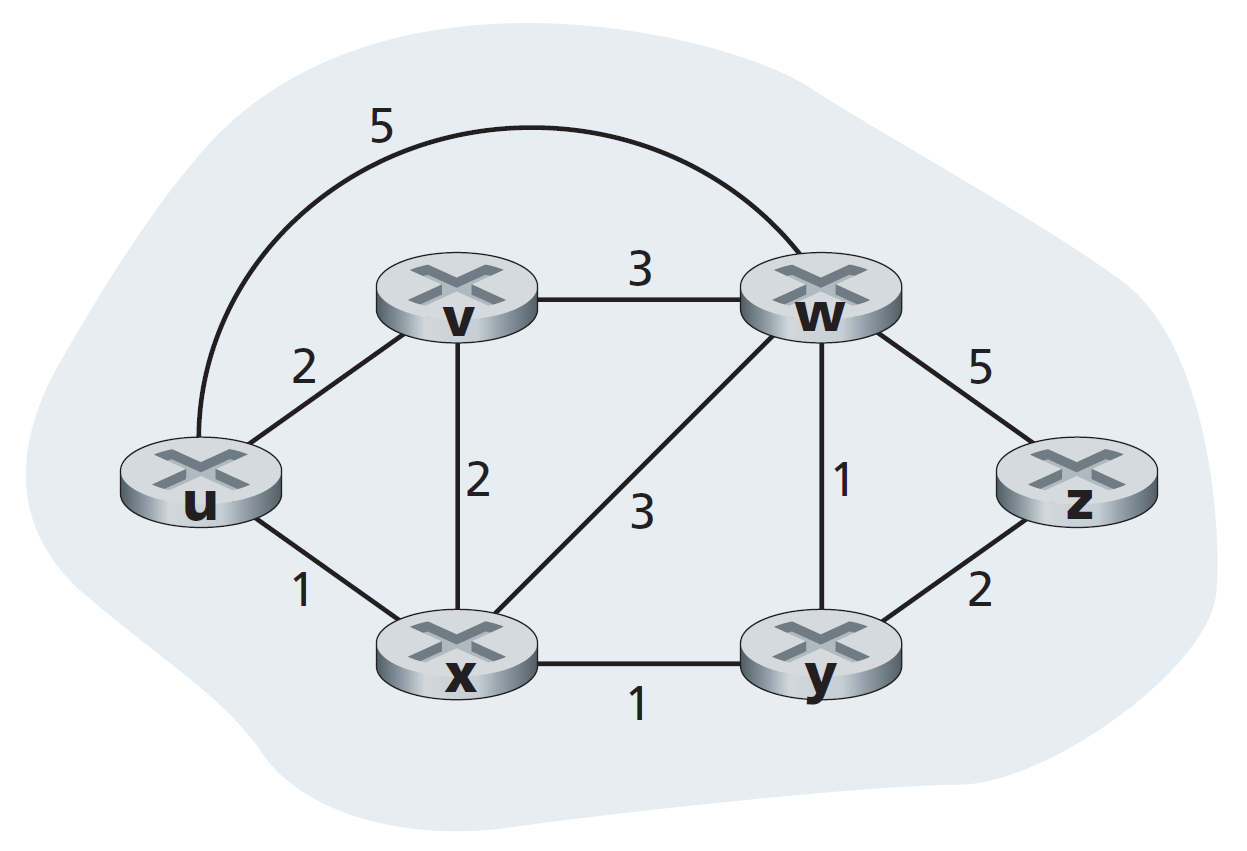
\includegraphics[keepaspectratio, width=12cm, height=9cm]{imagens/14/14 - grafo.png}
\caption{Grafo com pesos \\
Imagem retirada de: Computer Networking a top-down approach. 8th
ed.~Pearson, página 381. \\}
\label{fig:Grafo com pesos}
\end{figure}

As características de cada conexão (velocidade, tarifas financeiras,
etc.) são contabilizadas (a partir de métricas estabelecidas pela
instituição dona da rede), resultando no custo (ou peso) agregado à
conexão. Como cada aresta apresenta características diferentes, serão
agregados pesos diferentes ao uso de cada uma. Assim, os algoritmos de
roteamento, como o OSPF e o BGP (conhecido como a ``cola'' da Internet),
tem o objetivo de encontrar um caminho entre dois nós que apresente o
menor custo de ser percorrido (custo total do caminho).




É importante perceber que o caminho de menor custo (\emph{least-cost
path}) é diferente do caminho mais curto (\emph{shortest path}), pois o
primeiro é caracterizado por aquele que apresenta o menor somatório dos
pesos das conexões inseridas no mesmo, enquanto que o segundo é
determinado pela menor quantidade de nós que deve ser percorrido.

Ambos os algoritmos citados (OSPF e BGP) utilizam a abordagem
\emph{per-router control} (mostrado na Figura \ref{fig:Per Router Control}), em que o algoritmo de
roteamento é processado dentro de cada roteador, sendo necessário
interações entre \emph{routers} para a determinação das rotas. Outra
possível abordagem é a \emph{Logically centralized control} (mostrado na
Figura \ref{fig:Logically Centralized Controller}), em que há uma centralização computação em um servidor e
distribuição dos parâmetros determinados para os nós da rede, como
adotado pelo SDN (\emph{Software Defined Network}).


\begin{figure}[h!]
\centering
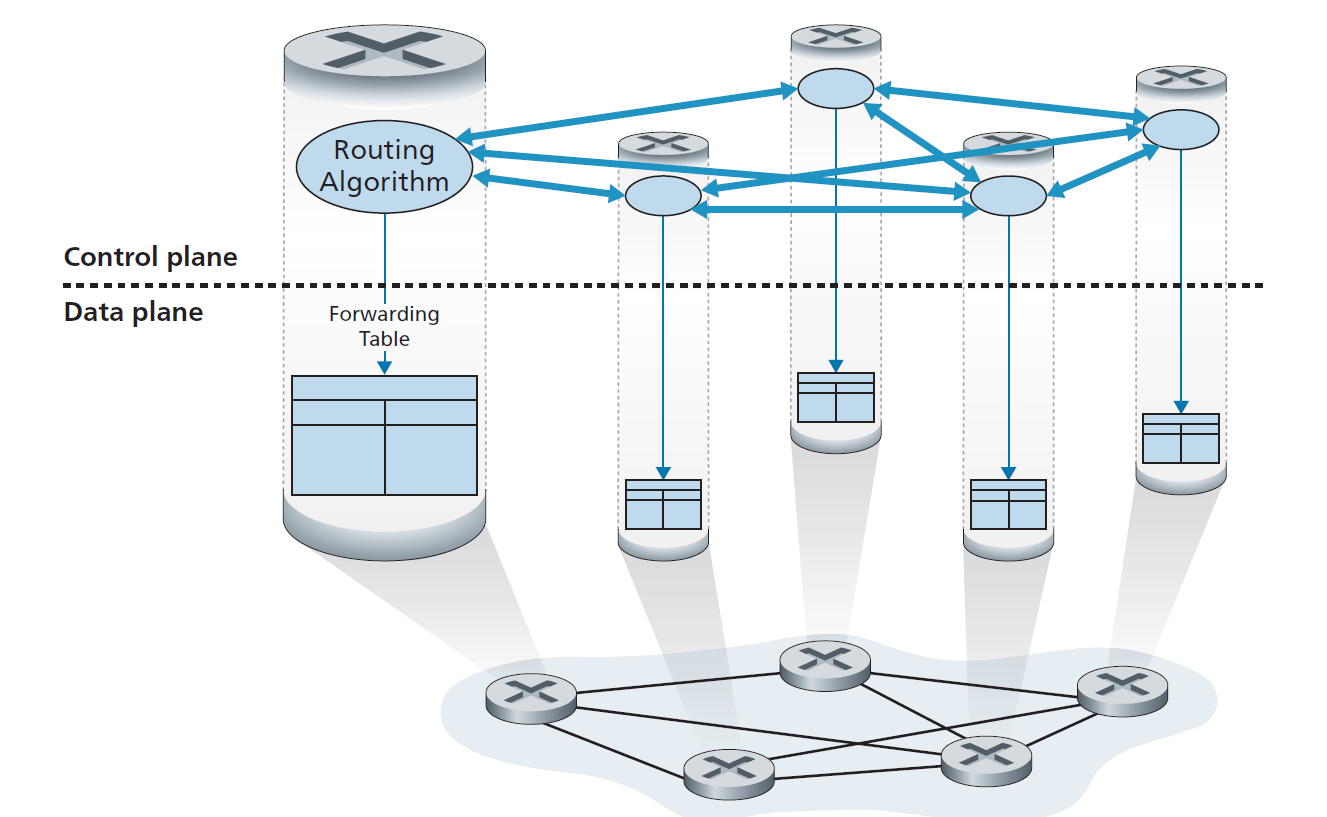
\includegraphics[keepaspectratio, width=12cm, height=9cm]{imagens/14/14 - per router control.png}
\caption{Per Router Control \\
Imagem retirada de: Computer Networking a top-down approach. 8th
ed.~Pearson, página 378. \\}
\label{fig:Per Router Control}
\end{figure}



\begin{figure}[h!]
\centering
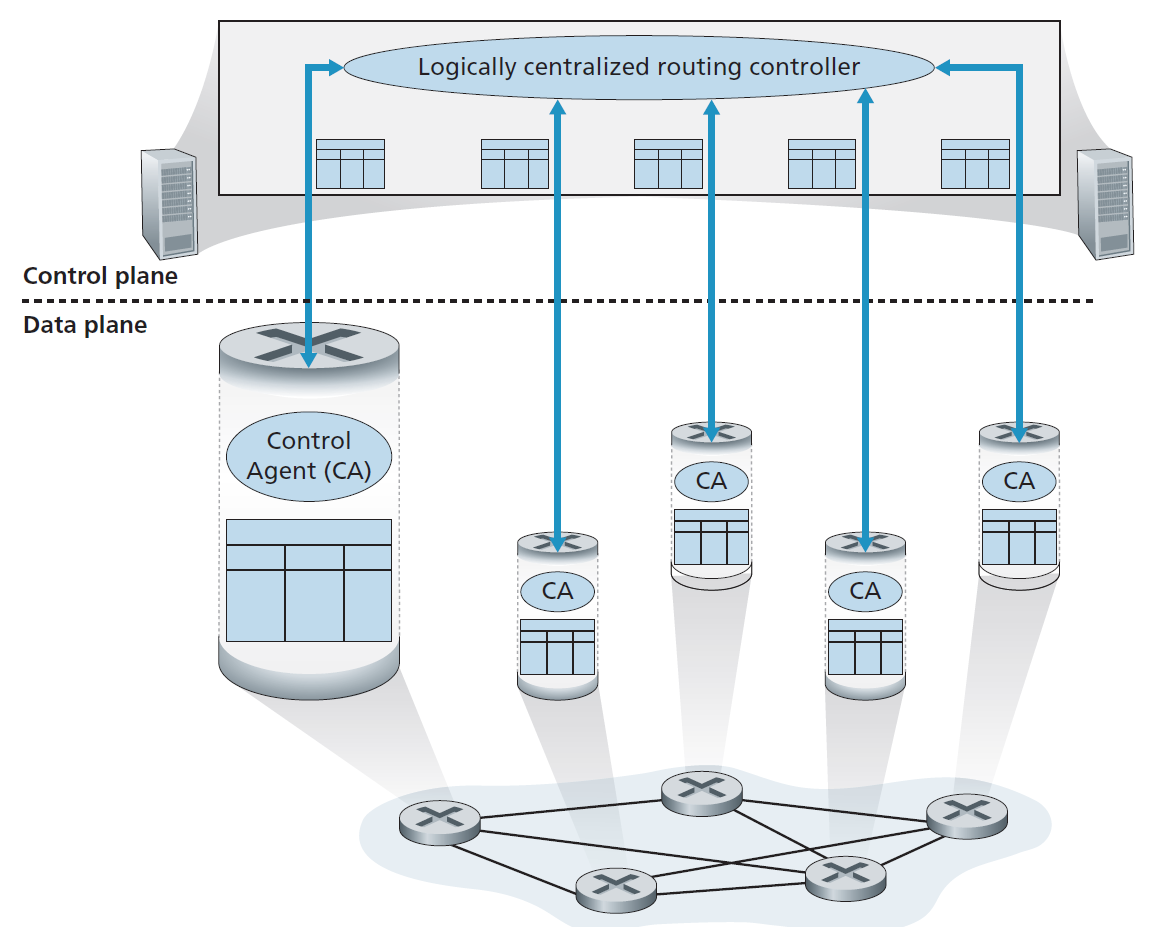
\includegraphics[keepaspectratio, width=12cm, height=9cm]{imagens/14/14 - Logically centralized controller.png}
\caption{Logically Centralized Controller \\
Imagem retirada de: Computer Networking a top-down approach. 8th
ed.~Pearson, página 379. \\}
\label{fig:Logically Centralized Controller}
\end{figure}




\hypertarget{Classificação dos algoritmos}{%
\section{Classificação dos algoritmos}\label{Classificação dos algoritmos}}

De forma abrangente, podemos classificar os algoritmos de roteamento em:

\begin{enumerate}
\def\labelenumi{\arabic{enumi}.}
\item
  \emph{Centralized routing algorithm}: os algoritmos dessa categoria,
  comumente referidos como \emph{link-state} (LS) \emph{algorithms},
  computam o caminho a partir de um conhecimento completo a cerca da
  conectividade e custos de cada conexão da rede (tendo um conhecimento
  global da rede). Um exemplo é o algoritmo de Dijkstra.
\item
  \emph{Decentralized routing algorithm}: a determinação do caminho de
  menor custo é feita de forma iterativa e distribuída em cada roteador.
  Como, inicialmente, cada roteador só têm conhecimento dos custos de
  seus próprios \emph{links}, o cálculo do menor caminho necessitará da
  troca de informações entre os outros roteadores da rede. Isso ocorre
  de forma iterativa e gradual. Um exemplo é o \emph{Distance-Vector
  Routing Algorithm} (DV), um algoritmo iterativo, assíncrono e
  distribuído, com cada nó mantendo um vetor de estimativas de custos de
  todos os outros nós da rede (com a atualização ocorrendo conforme
  mudanças na rede acontecem). Podemos citar alguns protocolos que
  utilizam o DV: Internet's RIP, BGP, ISO IDRP, Novel IPX e o original
  ARPAnet.
\end{enumerate}

Uma segunda forma de classificação é:

\begin{enumerate}
\def\labelenumi{\arabic{enumi}.}
\tightlist
\item
  \emph{Static Routing Algorithms}: os roteadores mudam muito pouco no
  decorrer do tempo (frequentemente como resultado de uma intervenção
  humana).
\item
  \emph{Dynamic routing algorithms}: as rotas mudam conforme a ocorre
  mudança na topologia da rede ou carga de tráfego (apesar dessa
  categoria apresentar maior responsividade em mudanças na rede, também
  estão mais suscetíveis a problemas como \emph{loops} e oscilações).
\end{enumerate}

Uma terceira forma:

\emph{Load-Sensitive algorithm}: os custos dos \emph{links} variam
dinamicamente conforme o nível de congestionamento.
\emph{Load-Insensitive algotihm}: os custos dos \emph{links} não
refletem explicitamente o nível de congestionamento.

\hypertarget{ls-vs-dv}{%
\section{LS vs DV}\label{ls-vs-dv}}

Alguns pontos são importantes para a comparação entre os
\emph{link-state algorithms} e o \emph{Distance-Vector Routing
Algorithm}:

\begin{enumerate}
\def\labelenumi{\arabic{enumi}.}
\item
  \emph{Message complexity}: o LS requer que cada nó saiba os custos de
  cada conexão da rede, com uma mudança em um custo devendo ser enviada
  para todos os nós. Já no DV, o envio do novo custo somente ocorre
  quando o mesmo impacta no caminho de menor custo dos nós anexados ao
  \emph{link} relativo à alteração (DV melhor que LS).
\item
  \emph{Speed of convergence}: LS converge mais rápido do que o DV (LS
  melhor que DV).
\item
  \emph{Robustness}: no DV, um caminho de menor custo calculado
  incorretamente por um nó será publicado para todos os nós da rede,
  diferentemente do LS, no qual os caminhos são calculados em cada nó,
  provendo assim um certo nível de robustez (LS melhor que DV).
\end{enumerate}

\hypertarget{intra-autonomous-sistems-routing-ospf}{%
\section{Intra-Autonomous Sistems Routing: OSPF}\label{intra-autonomous-sistems-routing-ospf}}

Um sistema autônomo (Autonomous Sistems, AS) consiste de um conjunto de
roteadores que estão sob um mesmo controle administrativo. Isso torna
possível a escalabilidade e a autonomia administrativa do sistema. Os
algoritmos de roteamento que rodam em um AS são chamados de
\emph{intra-autonomous system routing protocol}. Um exemplo de algoritmo
é o \emph{Open Shortest Path First}, um protocolo LS no qual as
especificações do protocolo de roteamento está disponível publicamente
(a parte \emph{Open} do nome). No OSPF, cada roteador monta um mapa
topológico completo de todo o AS, e então executa o algoritmo de
Dijkstra para a determinação da árvore de caminhos de menor custo para
todas as sub-redes, com os custos das conexões sendo configurados pelo
administrador da rede.

Observe que is roteadores que conectam-se com outros de diferentes ASs
são chamados de \emph{gateway routers} (eles estão nos limites da AS).
Já aqueles que estão no interior da AS, são chamados de \emph{internal
routers}.

Alguns pontos importantes de mencionar:

\begin{enumerate}
\def\labelenumi{\arabic{enumi}.}
\item
  \emph{Security}: as trocas de informações entre os roteadores OSPF
  podem ser autenticadas por meio da geração de um \emph{hash} MD5
  (utilizando-se uma chave secreta, que está contida no roteador e não é
  compartilhada) por ambos (emissor e receptor da mensagem). Em seguida
  o \emph{hash} do emissor é comparado com o do receptor. O emissor pode
  ser considerado autêntico caso os \emph{hashs} gerados sejam iguais.
  Caso contrário, a mensagem dese ser ignorada.
\item
  \emph{Multiple same-cost path}: O tráfego de dados poderá ser
  distribuído em todas as rotas que contenham o custo mínimo.
\item
  \emph{Support for hierarchy within a single AS}: o sistema pode ser
  configurado hierarquicamente em áreas.
\end{enumerate}

\hypertarget{inter-autonomous-sistems-routing-bgp}{%
\section{Inter-Autonomous Sistems Routing: BGP}\label{inter-autonomous-sistems-routing-bgp}}

Por necessitar a coordenação de múltiplos ASs, a comunicação entre ASs
deve ocorrer utilizando-se o mesmo protocolo. O protocolo usado é o
\emph{Border Gateway Protocol} (BGP), e é conhecido também por ser a
``cola'' da Internet (por unir os diferentes ASs).

O roteamento pelo BGP ocorre entre sub-redes e não para um endereço
específico da rede. Dessa forma, a \emph{forwarding table} do roteador
toma a forma de \texttt{(x,\ I)}, onde \texttt{x} é o prefixo e o
\texttt{I} é a interface do roteador.

O BGP provê para os roteadores meios para:

\begin{enumerate}
\def\labelenumi{\arabic{enumi}.}
\tightlist
\item
  Obter o prefixo de AS vizinhos: com a publicação da existência de cada
  rede para o resto da Internet.
\item
  Determinar a melhor rota para cada prefixo: no qual a melhor rota é
  baseada nas políticas determinadas pelo administrador da rede e na
  acessibilidade da informação.
\end{enumerate}

As conexões BGP entram em duas categorias (graficamente representado na
Figura \ref{fig:eBGP e iBGP}):

\begin{enumerate}
\def\labelenumi{\arabic{enumi}.}
\tightlist
\item
  iBGP (\emph{internal} BGP): conexão BGP internas aos ASs
\item
  eBGP (\emph{external} BGP): conexão externa aos ASs (entre ASs)
\end{enumerate}


\begin{figure}[h!]
\centering
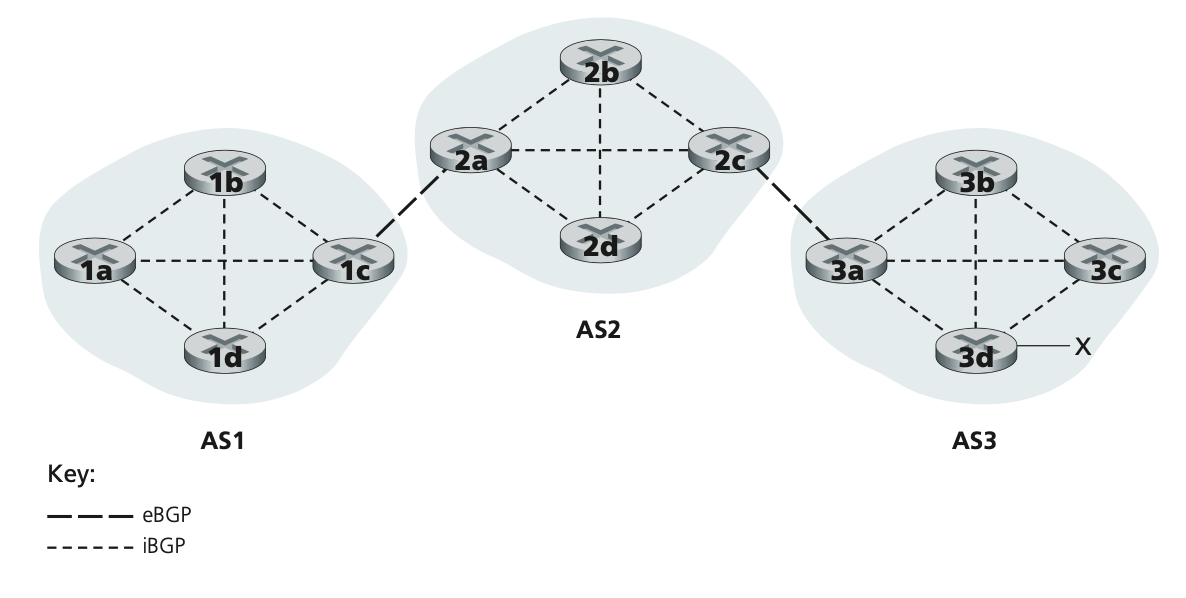
\includegraphics[keepaspectratio, width=12cm, height=9cm]{imagens/14/14 - eBGP e iBGP.png}
\caption{eBGP e iBGP \\
Imagem retirada de: Computer Networking a top-down approach. 8th
ed.~Pearson, página 402. \\}
\label{fig:eBGP e iBGP}
\end{figure}



A publicação no BGP ocorre de forma bem direta. A Figura \ref{fig:ASs com adição de x} mostra a
adição de uma sub-rede (\texttt{x}) em uma rede com 3 ASs. Primeiro o AS3
envia uma BGP \emph{message} (\texttt{AS3\ x}) para o AS2 dizendo que a
sub-rede \texttt{x} existe e é acessível através dele. Em seguida, o AS2
avisa para o AS1 a existência de \texttt{x} e que o mesmo é acessível
através do caminho AS2-AS3 (\texttt{AS2\ AS3\ x}).


\begin{figure}[h!]
\centering
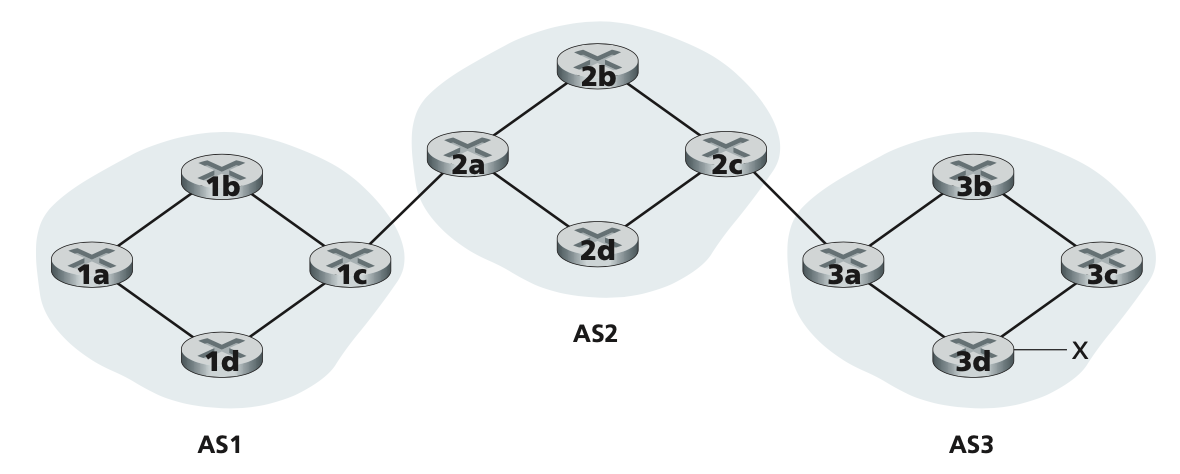
\includegraphics[keepaspectratio, width=12cm, height=9cm]{imagens/14/14 - SAs com a adicao de x.png}
\caption{ASs com adição de x \\
Imagem retirada de: Computer Networking a top-down approach. 8th
ed.~Pearson, página 401. \\}
\label{fig:ASs com adição de x}
\end{figure}



O BGP \emph{message} é composto pelo prefixo e outros múltiplos
atributos, como o \emph{AS-PATH}, que explicita a lista de ASs na qual a
mensagem publicação de existência da nova rede precorreu (como mostrado
no exemplo anterior), e \emph{NEXT-HOP}, que é o endereço da interface
do roteador que inicia a o \emph{AS-PATH}.

\hypertarget{hot-potato}{%
\section{Hot Potato}\label{hot-potato}}

Os ASs operam com a bordagem \emph{Hot Potato}, o qual os roteadores
objetivam transmitir os dados para fora do AS o mais rápido possível.
Para tal, o roteador com os dados disparará para o endereço do
\emph{NEXT-HOP} que tiver o menor custo de conexão, sem se preocupar com
o resto do trajeto desses dados. Assim, apesar de localmente eficiente,
a rota global escolhida pode não ser a mais rápida. A Figura \ref{fig:Duas possibilidades de NEXT-HOP} mostra
duas possibilidades de \emph{NEXT-HOP}. A rota escolhida será aquela que
apresentar o menor custo de conexão relacionado ao \emph{NEXT-HOP}. A
Figura \ref{fig:Passos para a adição de um destino externo na forwarding
table} mostra os passos para a adição de um destino externo ao AS na
\emph{forwarding table}

\begin{figure}[h!]
\centering
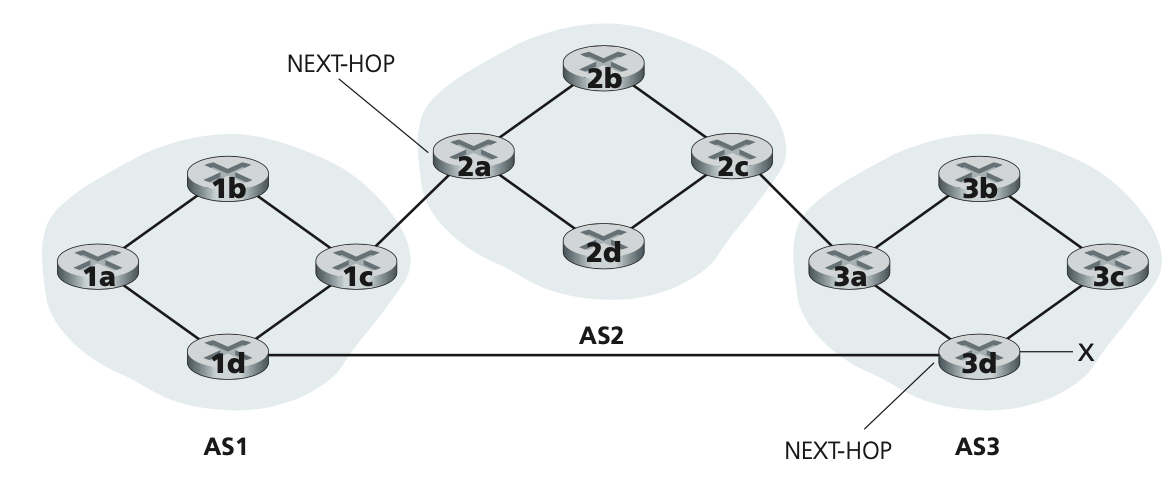
\includegraphics[keepaspectratio, width=12cm, height=9cm]{imagens/14/14 - rota com menor next-hop.png}
\caption{Duas possibilidades de NEXT-HOP \\
Imagem retirada de: Computer Networking a top-down approach. 8th
ed.~Pearson, página 403. \\}
\label{fig:Duas possibilidades de NEXT-HOP}
\end{figure}

\begin{figure}[h!]
\centering
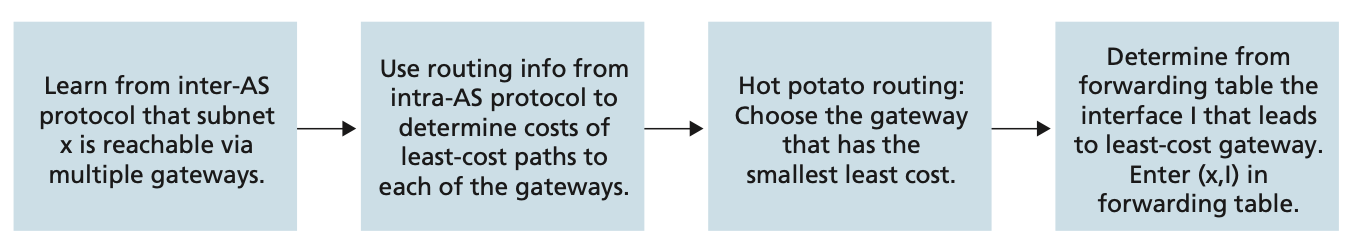
\includegraphics[keepaspectratio, width=12cm, height=9cm]{imagens/14/14 - adicao destino.png}
\caption{Passos para a adição de um destino externo na forwarding
table \\
Imagem retirada de: Computer Networking a top-down approach. 8th
ed.~Pearson, página 404. \\}
\label{fig:Passos para a adição de um destino externo na forwarding
table}
\end{figure}


\hypertarget{Seleção da rota.}{%
\section{Seleção da rota.}\label{Seleção da rota.}}

Na prática, a rota selecionada utiliza outros parâmetros além do
\emph{Hot Potato}:

\begin{enumerate}
\def\labelenumi{\arabic{enumi}.}
\tightlist
\item
  Política de decisão da preferência local de transmissão: essa política
  é escolhida pelo administrador da rede
\item
  Para os restantes, será escolhido o que tiver o menor \emph{AS-PATH}.
\item
  Para os restantes, o \emph{Hot Potato} entra em ação, escolhendo a
  rota com o menor custo de transmissão para o \emph{NEXT-HOP}.
\item
  Para os restantes, é utilizado os identificadores BGP para a seleção
  da rota.
\end{enumerate}

\hypertarget{poluxedtica-de-preferuxeancia-local-e-protocolos-intra-vs-inter}{%
\section{Política de preferência local e Protocolos Intra vs Inter}\label{poluxedtica-de-preferuxeancia-local-e-protocolos-intra-vs-inter}}

O AS é dito como sistema autônomo pois o mesmo apresenta uma
independência administrativa. Isso é algo que pode gerar alguns
problemas de confiança, com decisões como não permitir que dados
originário de um AS passe através de outro AS específico. E, de forma
similar, um AS pode ter interesse em querer controlar o tráfego de dados
entre outros ASs. Um reflexo no cenário atual é a desconfiança dos
americanos sob empresas chinesas, que, comumentemente, recebe
interferência do governo chinês, um inimigo declarado dos EUA (assim,
deve-se ser evitado que dados críticos do governo americanos sejam
transmitidos através de empresas chinesas).

Outra questão gira em torno do problema de uma sub-rede de um cliente
fazer parte da rota dos dados de outros clientes. Um cliente deve ser
origem ou destino das mensagens e não um meio.

A política é uma questão tão forte na comunicação inter-ASs, que ela é
um dos maiores motivos para que os protocolos inter-ASs sejam diferentes
dos intra-ASs, tanto que até a qualidade das rotas (externas) utilizadas
é uma preocupação secundária. Por fim, a questão da escala não é tão
forte no intra-ASs quanto é em inter-ASs. Assim, os 3 motivos para que
os protocolos sejam diferentes são:

\begin{enumerate}
\def\labelenumi{\arabic{enumi}.}
\tightlist
\item
  Política: intra-ASs é secundário, inter-ASs é primário.
\item
  Escala: intra-ASs é secundário, inter-ASs é primário.
\item
  Performance: intra-ASs é primário, inter-ASs é secundário (impactado
  pelas políticas).
\end{enumerate}